\chapter{Probabilistic Modeling}

\section{Modeling with Probability Distributions}

% a discussion on binomial distribution.
The normal rate of infection of a certain disease in cattle is
25\%.  Each animal becomes infected (or not) independently of other
animals.  A team of veterinarians would like to test a new
vaccine. Which of the following two scenarios, \ref{sc1} or \ref{sc2},
provides more evidence that the vaccine is effective.  \emph{Hint:}
Compute the probability that each scenario would occur under the
hypothesis that the vaccine has no effect whatsoever.
\begin{enumerate}[A)]
\item 10 animals are vaccinated and none of them become infected. \label{sc1}
\item 17 animals are vaccinated. At most one of the animals becomes infected. \label{sc2}
\end{enumerate}

Let $X$ be the number of animals infected under the assumption that
the vaccine is worthless.  Under scenario \ref{sc1},
\[ X \sim \text{Binomial}(n=10,p=.25) \]
\[ P(X = 0) = {10 \choose 0} .25^0 .75^{10} = .0563 \]
Under scenario \ref{sc2}, 
\[ X \sim \text{Binomial}(n=17,p=.25) \]
\begin{align*} P(X \leq 1) &= P(X=0) + P(X=1) \\
                 &= \sum_{x=0}^1 {17 \choose x} .25^x .75^{17-x} \\
                 &= .0501
\end{align*}
In the absence of a working vaccine, scenario \ref{sc2} is less likely to occur,
and so it provides a better test of the effectiveness of the vaccine.


% use this section to illustrate modeling with a poisson rv
At a facility that manufactures recreational sports
  vehicles (ATVs), each vehicle is subjected to a final
  inspection. The rate of defects during final inspection is
  $\lambda=1.5$ defects per vehicle.
\begin{enumerate}
\item What is an appropriate probability distribution to model the
number of defects? \label{atv1}
\item What proportion of vehicles have more than 2 defects? \label{atv2}
\item Management has set a new goal that the proportion
of vehicles with no defects is .5. What rate $\lambda$ would
achieve this goal? \label{atv3}
\end{enumerate}

We are interested in the number of defects, which is discrete.
The Poisson distribution makes sense because it is commonly used
for count data. Moreover, we are given information for a single
parameter, and the Poisson distribution has a single parameter.
If we let the random variable $X$ represent the number of defects
per vehicle, then a reasonable distribution is
\[ X \sim \text{Poisson}(\lambda=1.5) \]
For part~\ref{atv2},
\begin{align*}
P(X>2) &= 1 - P(X \leq 2)\\
       &= 1 - \sum_{x=0}^2 \frac{e^{-\lambda}\lambda^x}{x!}\\
       &= 0.191
\end{align*}
For part \ref{atv3}, management's goal is that $P(X=0)=0.5$, or
\[ P(X=0) = \frac{e^{-\lambda}\lambda^0}{0!} = e^{-\lambda}=0.5 \]
Then
\[ \lambda = -\ln{0.5} = 0.693 \]

%% using poisson distribution and binomial distribution, and independence
The number of bacteria colonies of a certain type in samples of
polluted water has a Poisson distribution with a mean of 2 per cubic
centimeter. If four 1--cubic--centimeter samples are independently
selected from this water, find the probability that at least one
sample will contain one or more bacteria colonies.

Let $X$ be a random variable that represents the number of bacteria
colonies in a 1 cm$^3$ sample of the polluted water. From the problem
description,
\[ X \sim \text{Poisson}(\lambda = 2) \]
First let's find the probability that any particular sample will contain
at least one colony.
\begin{align*}
  P(X \geq 1) &= 1 - P(X=0)\\
              &= 1 - \frac{e^{-\lambda}\lambda^0}{0!}\\
              &= 1 - e^{-2}\\
  &= .865
\end{align*}
Now, the four samples are independent and the the probability that
a sample contains one or more colonies is the same for each sample.
Let $Y$ be a random variable that represents the number of samples
that contain one or more colonies. Then
\[ Y ~ \sim \text{Binomial}(n=4, p=0.865) \]
and we want to know $P(Y \geq 1)$.
\begin{align*}
  P(Y \geq 1) &= 1 - P(Y = 0)\\
              &= 1 - {4 \choose 0} (.865)^0 (1 - .865)^4 \\
  &= 0.9997
\end{align*}

% discussion on the Normal distribution
A refinery makes two grades of gasoline, regular and premium.  The
advertised octane ratings are 87 for regular gasoline and 89 for
premium gasoline.  The quality engineer at the refinery asks for 10
samples from one of the two types of gasoline. She does not know for
sure whether the samples are from the regular batch or the premium
batch. She devises the hypothesis test
\begin{align*}
H_0: \mu &\leq 87 \\
H_1: \mu &> 87
\end{align*}
and sets the confidence level to be 0.995. Suppose that the mean of
the 10 samples is 88.3 and the standard deviation is 1.0. What is her
conclusion for the hypothesis test?

Suppose that a gas station owner has his own octane test
kit and rule for accepting a tanker-truck of premium gasoline.
The owner knows from past shipments that the distributions
of octane ratings are
\begin{align*}
X_{\text{regular}} &\sim N(87,1) \\
X_{\text{premium}} &\sim N(89,1)
\end{align*}
Although the owner may not think about it explicitly, his hypothesis
test is
\begin{align*}
H_0: \mu &= 87 \\
H_1: \mu &= 89
\end{align*}
The owner takes one sample from the tanker-truck. If the octane
measurement is greater than 88.5, then he will accept the shipment as
premium gasoline. What is the probability that the owner accepts a
shipment of regular gasoline as premium (i.e. what is $\alpha$)? What
is the probability that he declines a shipment of premium gasoline,
claiming that he thinks it is regular (i.e. what is $\beta$)?  Use the
Normal distribution for this problem. The following diagram may help.

\begin{tikzpicture}
\begin{axis}[
  no markers, domain=0:12, samples=100,
  height=5cm, width=15cm,
  axis x line=bottom,
  axis y line=none,
  xtick=\empty, ytick=\empty,
  extra x ticks={4,6,7},
  extra x tick labels={87,88.5,89},
  enlargelimits=false, clip=false
  ]
  
  \addplot [fill, pattern=north west lines, domain=0:6] {gauss(7,1)} \closedcycle;
  \addplot [fill, draw=none, domain=6:12] {gauss(4,1)} \closedcycle;
  \addplot [thick] {gauss(4,1)};
  \addplot [thick] {gauss(7,1)};

  \draw [ultra thin] (4,0) -- (4,.3989);
  \draw [ultra thin] (7,0) -- (7,.3989);

  \draw (4,.42) node[anchor=south] {$H_0$};
  \draw (7,.42) node[anchor=south] {$H_1$};

  \draw (4.9,.15) node[anchor=east] (beta) {$\beta$};
  \draw (5.4,.03) node (beta2) {};
  \draw[-] (beta) -- (beta2);

  \draw (6.5,.15) node[anchor=west] (alpha) {$\alpha$};
  \draw (6.1,.005) node (alpha2) {};
  \draw[-] (alpha) -- (alpha2);
  
\end{axis}
\end{tikzpicture}

For the quality engineer, the test statistic is
\[
t_0 = \left( \overline{X} - \mu_0 \right)\frac{\sqrt{n}}{S} 
= \left(88.3 - 87\right) \frac{\sqrt{10}}{1} 
 = 4.11
\]
and since $t_0 > t_{\alpha,n-1}=3.25$ ($\alpha=0.005$) she will
reject $H_0$ and conclude that the samples are from the premium
batch of gasoline.

For the station owner,
\begin{align*}
\alpha &= P(X > 88.5 \mid H_0) \\
&= P\left( Z > \frac{88.5-87}{1} \right) \\
&= 1 - P(Z < 1.5) \\
&= 0.067
\end{align*}
and
\begin{align*}
\beta &= P(X < 88.5 \mid H_1) \\
&= P\left( Z < \frac{88.5-89}{1} \right) \\
&= P(Z < -0.5) \\
&= 0.309
\end{align*}


\section{Stochastic Processes}

% Use this section to introduce the idea of a Poisson Process.
% add explanatory material.
\emph{A Poisson Process.} A statistician has observed the behavior of
a Hollywood celebrity for about one year and has noted that between
the hours of 8pm and 11pm this celebrity generates, on average, three
tweets per hour and that the rate is approximately the same within
each one-hour period.  We can count the \emph{number} of tweets that
occur in a time interval $t$. We can also measure the \emph{time}
between tweets. Here is a depiction of the tweets from last night.

\vspace{.2in}
\begin{center}
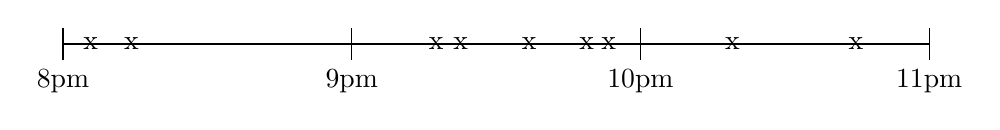
\begin{tikzpicture}

\draw (0,0) -- (11,0)
  node[pos=0.35/11]{x}
  node[pos=0.87/11]{x}
  node[pos=4.74/11]{x}
  node[pos=5.05/11]{x}
  node[pos=5.92/11]{x}
  node[pos=6.65/11]{x}
  node[pos=6.93/11]{x}
  node[pos=8.50/11]{x}
  node[pos=10.07/11]{x}
;
\node[below] at (0,-.2) {8pm};
\draw (0,-.2) -- (0,.2);
\node[below] at (11/3,-.2) {9pm};
\draw (11/3,-.2) -- (11/3,.2);
\node[below] at (22/3,-.2) {10pm};
\draw (22/3,-.2) -- (22/3,.2);
\node[below] at (11,-.2) {11pm};
\draw (11,-.2) -- (11,.2);


\end{tikzpicture}
\end{center}

Let the random variable $Y$ be the number of tweets from
the celebrity in some time interval.
When we say that the number of tweets in a time interval $t$ follows
a Poisson distribution with mean $\lambda t$, we write
\[
  Y \sim \text{Poisson($\lambda t$)}
\]
If $t$ is one hour, then we can write
\[
  Y \sim \text{Poisson($\lambda = 3$)}
\]
Stating that the number of tweets follows a Poisson distribution
implies that the time between tweets follows an Exponential
distribution (and vice versa). Let the random variable $X$ be
the time between tweets. Then
\[
  Y \sim \text{Poisson($\lambda t$)} \Longleftrightarrow X \sim \text{Exp($\lambda$)}
\]
Yes, it is the same $\lambda$ in each distribution.
The average number of tweets is $\lambda=3$ per hour. The average
time between tweets is $1/\lambda = 1/3$ hour (or 20 minutes).
Recall that for the Exponential distribution
\[
  E(X) = \frac{1}{\lambda} = \frac{1~\text{hour}}{3~\text{tweets}} = 20 ~\text{minutes per tweet on average}
\]

Questions.
\begin{enumerate}
\item What is the probability that the celebrity sends out five or
  more tweets in one hour?
\item What is the probability that the celebrity sends out
  no tweets between 9pm and 11pm?
\end{enumerate}

\section{Queueing Models}

\section{Exercises}

\begin{enumerate}
  
\subsubsection*{Modeling with Probability Distributions.}

% this problem is OK
% geometric distribution
\item \emph{Searching for an item.} Albert has \num{1176} Pok\'{e}mon
  cards in total.  Pok\'{e}mon EX is a special type of card, and
  Albert has 39 EX-type cards.  He is looking for an EX-type card, but
  all of the cards are completely mixed up and stored in a shoe
  box. His mother is calling him for dinner.  What is the probability
  that Albert will have to look through no more than 25 cards before
  he finds an EX-type card?

\begin{solution}
\bs Consider finding an EX-type card to be a ``success''. Let $X$ be a
random variable that represents the number of cards that Albert has to
handle up to and including the first success. Then
\[
X \sim \text{Geometric}(p=\frac{39}{1176})
\]
and
\[
P(X \leq 25) = 1 - (1 - p)^{25} \approx 0.57.
\]
\end{solution}

% this problem is OK
% Binomial, odds, probabilities
\item \emph{Playing Pok\`{e}mon.} Albert is playing
  Pok\'{e}mon cards with his friend. It's Albert's turn, and he
  decides to use Marowak. The card says the following.
\begin{quote}
\emph{Flip a coin four times. The amount of damage done to your opponent's
Pok\'{e}mon is the number of heads times 40.}
\end{quote}
What are the odds that Marowak will do at least 120 damage to the
opponent? One approach to answer this question is to use the Binomial
distribution to compute the probability of doing at least 120 damage
and then convert from probability to odds. You can take another
approach if you prefer. In any case, assume that the coin is fair,
i.e.\ the probability of getting heads on any particular toss is 1/2.

\begin{solution}
\bs
In order to do at least 120 damage, we need either three or four heads
out of the four coin tosses. Let $X$ represent the number of heads obtained
in four tosses of a fair coin. Then $X \sim \text{Binomial}(p=1/2,n=4)$.
\begin{align*}
P(X=3) + P(X=4) &= {4 \choose 3} p^3 (1-p)^1 + {4 \choose 4} p^4 (1-p)^0 \\
&= \frac{1}{4} + \frac{1}{16} \\
&= \frac{5}{16}
\end{align*}
The odds are
\[
\frac{p}{1-p} = \frac{\frac{5}{16}}{1-\frac{5}{16}} = \frac{5}{11}
\]
or 5 to 11.
\end{solution}

% this problem needs to be re-written
% binomial distribution
\item A power utility can supply electricity to a city
from $n$ different power plants. Each power plant fails with
probability $p$, independent of the others.
\begin{enumerate}
\item Suppose that any one plant can produce enough electricity to
supply the entire city. What is the probability that the city will
experience a black-out? \label{p1}
\item Suppose that two power plants are necessary to keep the city
from a black-out. Find the probability that the city will
experience a black-out. Simplify your answer for full credit.
\label{p2}
\end{enumerate}

\begin{solution}
\bs
For part~\ref{p1}, all $n$ plants must fail for the city to
have a black-out. Since failures are independent, the probability
of a black-out is $p^n$.

For part~\ref{p2}, let $X$ be the number of failed plants. $X$
has a Binomial distribution with parameters $n$ and $p$. The probability
of a black-out is
\begin{align*}
  P(X \geq n-1) &= \sum_{i=n-1}^n {n \choose i} p^i (1-p)^{n-i} \\
                &= {n \choose n-1} p^{n-1} (1-p)^{n-(n-1)} + {n \choose n} p^n (1-p)^{n-n} \\
                &= np^{n-1}(1-p) + p^n \\
                &= np^{n-1} - np^{n-1}p + p^n\\
                &= np^{n-1} - np^n + p^n\\
                &= np^{n-1} + (1-n)p^n
\end{align*}
\end{solution}

% this problem is OK
% exponential distribution
\item \emph{Evaluating a warranty.}
  A manufacturer of automotive batteries offers a one-year
  warranty. If the battery fails for any reason during the warranty
  period, it is replaced for free. The time to failure is distributed
  Exponential with rate $\lambda=.125$ failures per year.
\begin{enumerate}
\item What proportion of batteries fail within the warranty period?
\item The cost to manufacture a battery is \$50, and the profit
per battery is \$25. What is the effect of the warranty replacement
policy on profit? \label{ex:profit}
\end{enumerate}

\begin{solution}
  \bs The question is asking for the theoretical proportion of
  batteries that fail within one year. Since all batteries have the
  same probability of failure, this proportion is equal to the
  probability that a single battery will fail within one year. Let $X$
  be a random variable that represents the time to failure.
\[ P(X<1) = 1-e^{-\lambda t} = 1 - e^{-.125} = 0.118 \]
Now, imagine that the manufacturer has, over time,
  sold many batteries and has kept data on how many batteries failed
  within one year. The empirical proportion is simply the number
  of batteries that failed divided by the number of batteries sold.
  The Law of Large Numbers tells us that when the number of batteries
  sold is large, the empirical proportion will be approximately
  equal to the theoretical proportion.

Taking the warranty into account, the average profit per battery is
\[ \$25 - 0.118\times \$50 = \$19.10 \]
So, the (average) effect of the warranty on profit is -\$5.90.
\end{solution}

% memoryless property of the Exponential distribution this problem is
% from Ross. It's a thought experiment. The actual numbers don't
% matter as long as the rates are the same. Can we find a different
% scenario that illustrates the same idea: the memoryless property
\item \emph{Memoryless property of the Exponential distribution.}
  There are two clerks at the local post office. You enter the post
  office to find that both clerks are busy (i.e. each clerk is serving
  a customer), but that no one is in line.  So, you are first in line
  and you are to be served by the first available clerk. Customers
  depart the post office as soon as they are finished being served by
  a clerk. If the service time distribution for each clerk is
  Exponential with rate $\lambda$, what is the probability that you
  are the last of the three customers to depart the post office?

\begin{solution}
\bs
By the memoryless property of the Exponential distribution, the
remaining time for each customer currently being served is identical.
In particular, if we let $Y$ be the remaining time of a customer, then
the distribution of remaining time is
\[ P(Y \leq y) = 1 - e^{-\lambda y} \] Since the two customers have
the same distribution for remaining time, the probability that
customer 1 departs before customer 2 is 1/2 (likewise for
customer 2 departing before customer 1). When you enter service, the
memoryless property still applies.  Regardless of how long the
other customer has been in service, you have the same distribution
for remaining time. So, the probability that you are the last to depart
is 1/2.
\end{solution}

% this problem has been re-written
% Poisson distribution
\item \emph{Donut giveaway.}  A professional baseball team has just
  won a game that secured them a berth in the league’s playoffs. To
  celebrate, a local donut shop will be giving away up to 200 free
  donuts during a two-hour period on the morning following the
  victory. All 200 donuts will be baked and decorated with a baseball
  theme before the giveaway starts. If there are any donuts remaining
  after the giveaway, they will be sold at a discounted price. Assume
  that customers will arrive at the giveaway according to a Poisson
  process at a mean rate of 100 customers per hour. Also, note that
  there is a limit of one donut per customer.
\begin{enumerate}
\item What is the probability that there will be donuts remaining after the giveaway? \label{ex:donuta}
\item What is the predicted number of donuts that will be remaining after the giveaway? \label{ex:donutb}
\end{enumerate}

For part~\ref{ex:donuta}, present your answer as an expression for the
probability that there will be donuts remaining. Then, use software,
such as R, to compute a numerical answer.

\begin{solution}
  \bs Given that customers arrive to the giveaway according to a
  Poisson process with a mean of 100 customers per hour, the number of
  customers that arrive during the two-hour period is Poisson
  distributed with a mean of 200. Let $N$ be the number of customers
  arriving in a two-hour period. Then
\[ N ~ \text{Poisson}(\lambda = 200) \]
For part~\ref{ex:donuta}, the probability that there will be donuts remaining after the giveaway is 
\begin{align*}
      P(N < 200) &= \sum_{n=0}^{199} \frac{\lambda^n e^{-\lambda}}{n!}\\
      &= \sum_{n=0}^{199} \frac{200^n e^{-200}}{n!}\\
      &\approx .49
\end{align*}
In R,
\begin{Verbatim}
> sum(dpois(0:199,200))
[1] 0.4905966
\end{Verbatim}  

For part~\ref{ex:donutb}, our calculations are all done in expectation
(that is to say, on average). There are 200 customers in 2 hours,
which means that 200 donuts are given away. So, on average, no donuts
are remaining.
\end{solution}

% re-written by hannah
% Poisson distribution
\item \emph{Startup expenses.}  Two friends are starting a small
  business selling ice cream. They applied for a grant and have
  received \$\num{1800} to help cover any startup expenses. The
  friends will incur expenses of \$300 randomly throughout the first
  year, and the time between payments for these expenses is
  exponential with a mean of 2 months. Determine the probability that
  the friends will run out of grant money before the end of the year.

\begin{solution}
  \bs Let $X$ be a random variable that represents the time between
  payments. The mean time between payments, that is to say the
  expected value of $X$ ($E(X)$), is two months. We know that for the
  Exponential distribution
  \[ E(X) = \frac{1}{\lambda} \] where $\lambda$ is the rate (in units
  of payments per month). So,
  \[ X \sim \text{Exp}(\lambda = 1/2~\text{payments per month}) \] If
  the time between payments is distributed Exponential with rate
  $\lambda$, then the number of payments in $t$ months is Poisson with
  mean $\lambda t$. Let $N$ be the number of payments in 12 months.
  \[ N \sim \text{Poisson}(\lambda t = \lambda \times 12 = 6) \] Now,
  the probability that the friends runs out of money is
\begin{align*}
      P(N \geq 6) &= 1 - P(N \leq 5) \\
      &= 1 - \sum_{n=0}^{5} \frac{\lambda^n e^{-\lambda}}{n!}\\
      &= 0.55
\end{align*}
You may have defined the event that the friends runs out of
money as $P(N = 6)$. In other words, that there are exactly
six payments during the first year.  This is incorrect because
we are modeling the spending activity as a Poisson process. In
other words, the (unstated) assumption is that the number of
payments is independent of the available funds.
\end{solution}

% re-written by hannah
% poisson distribution
\item \emph{Stocking a vending machine.}  A university cafeteria has a
  vending machine that is stocked with a variety of juices and
  sodas. A vending machine attendant replenishes inventory weekly so
  that there are 180 beverages in stock at the beginning of each
  week. The cafeteria is open 24 hours, 7 days a week, and it is
  expected that the beverages will be purchased according to a Poisson
  distribution with a mean of 1 hour between purchases.
\begin{enumerate}
\item What is the probability that there are no beverages remaining in
  the vending machine when the attendant arrives? \label{ex:pout}
\item On average, how many beverages will be remaining in the vending
  machine when the attendant arrives? \label{ex:qremain}
\item What is the probability that the attendant will replenish 150 or
  more beverages? \label{ex:preplenish}
\end{enumerate}

\begin{solution}
  \bs For part~\ref{ex:pout}, there will be no beverages remaining in
  the vending machine if demand for beverages is at least 180.
  Because the beverages are purchased according to a Poisson
  distribution with a mean of one hour between purchases, the rate
  $\lambda$ that beverages are purchased is 24 beverages per
  day. Therefore, the number of purchases in seven days is Poisson
  with mean $\lambda t$. Let $N$ be a random variable that represents
  the number of purchases in one week (seven days).
  \[ N \sim \text{Poisson}(\lambda = \lambda \times 7 = 168) \] 
\begin{align*}
      P(N \geq 180) &= 1 - P(N \leq 179)\\
      &= 1 - \sum_{i=0}^{179} \frac{168^i e^{-168}}{i!}\\
      &\approx 0.19
\end{align*}
In R,
\begin{Verbatim}
> 1 - sum(dpois(0:179,168))
[1] 0.1866995
\end{Verbatim}

For part~\ref{ex:qremain}, the expected number of purchases from the
vending machine each week is 168 beverages. Therefore, the expected
number of beverages remaining at the end of the week is $180-168=12$.
	
For part~\ref{ex:preplenish}, 150 or more beverages will be
replenished if 150 or more beverages are purchased before the end of
the week. The probability that 150 or more beverages are purchased
during a week is
\begin{align*}
      P(N \geq 150) &= 1 - P(N \leq 149)\\
      &= 1 - \sum_{i=0}^{149} \frac{168^i e^{-168}}{i!}\\
      &\approx 0.93
\end{align*}
In R,
\begin{Verbatim}
> 1 - sum(dpois(0:149,168))
[1] 0.9253016
\end{Verbatim}
\end{solution}

% this problem needs to be re-written.
% Poisson distribution
\item \emph{Car dealership.} A car dealership keeps 200 used cars that are for sale in an uncovered parking lot. In the city where the dealership is located, hailstorms occur randomly throughout the month of June according to a Poisson distribution with a mean of 4 hailstorms. During a hailstorm, the number of cars that are damaged follows a Poisson distribution with a mean of eight damaged cars per 10 cars in the parking lot.
\begin{enumerate}
	\item Determine the probability that there will be exactly 5 hailstorms at the dealership in June. \label{a}
	\item During a hailstorm, determine the probability that 170 or more cars will be damaged. \label{b}
\end{enumerate}

\begin{solution}
	\bs For part~\ref{a}, let $X$ be a random variable that represents the number of hailstorms in June. The number of hailstorms in June follows a Poisson distribution with a mean of 4 hailstorms. Therefore, $X \sim \text{Poisson}(\lambda = 4)$.
	
	The probability that there are exactly 5 hailstorms is 
	\[
	P(X=5) = \frac{e^{-\lambda}\lambda^5}{5!} = \frac{e^{-4}4^5}{120} \approx 0.16
	\]
	For part~\ref{b},the rate that cars are damaged is Poisson with a mean of 8 damaged cars per 10 cars in the parking lot. Let $N$ be the number of damaged cars in the parking lot when 200 cars are present.
	\[ N \sim \text{Poisson}(\lambda = 160) \] 
	
	The probability that 170 or more cars will be damaged in a hailstorm is 
	\begin{align*}
		P(N \geq 170) &= 1 - P(N \leq 169) \\
		&= 1 - \sum_{n=0}^{169} \frac{\lambda^n e^{-\lambda}}{n!}\\
		&\approx 0.22
	\end{align*}
	Using R,
	\begin{Verbatim}
	> 1 - sum(dpois(0:169,160))
	[1] 0.2245714
	\end{Verbatim}
\end{solution}

% this problem is OK
% a poisson process, memory-less property of exponential distribution
\item A dump truck at a mine takes ore to the railroad after 10
  one-ton scoops have been loaded into the truck.  The one-ton scoops
  are loaded from a large diesel-powered shovel independently and at a
  mean rate of seven scoops per hour.  The time between scoops from the
  shovel can be considered to follow an Exponential distribution.

\begin{enumerate}
\item Find the probability that the time between consecutive trips to
  the railroad will be at least one hour.
\item It takes the dump truck 18 minutes to travel to the railroad,
  unload, and return. Suppose the truck returns and finds that no
  scoop is ready to be loaded. What is the probability that the next
  scoop is ready within 5 minutes? \label{item:2}
\end{enumerate}

\begin{solution}
  \bs The time between scoop arrivals is distributed Exponential, so
  we know that the number of arrivals in a time interval is
  distributed Poisson. In particular, the number of arrivals in a
  one-hour period follows a Poisson distribution with mean
  $\lambda=7$. In order for the time between consecutive trips to the
  railroad to take at least one hour, we require that the number of
  arrivals in one hour is nine or less. Let $X$ be the number of
  (scoop) arrivals in a one hour period.
\[
P(X \leq 9) = \sum_{x=0}^9 \frac{e^{-\lambda}\lambda^x}{x!} = .83.
\]
For part \ref{item:2}, we can invoke the memoryless property of the
Exponential distribution. The remaining time until the next arrival is
disitributed Exponential with rate 7 scoops per hour, regardless of how
much time has elapsed since the last arrival. Let $Y$ be the time
until the next arrival, and don't forget to convert from minutes to
hours.
\[
P(Y \leq 5) = 1 - e^{-7\times \frac{5}{60}} = .44
\]
\end{solution}

% this problem needs to be re-written
% normal distribution
\item Normal distribution. High blood pressure is an underlying health condition that makes people more susceptible to severe illness. A company conducted blood pressure screenings to determine the risk its employees have for severe illness. The systolic blood pressure $x$ of 220 employees was measured, and the mean blood pressure was 135 with a standard deviation of 20. The company doctor has created the following guidelines for determining which employees are at highest risk.

\begin{tabular}{lc}
	systolic blood pressure & risk \\ \hline
	$\mu+1.5\sigma < x$ & very high \\
	$\mu < x < \mu+1.5\sigma$ & high \\
	$\mu-\sigma < x < \mu$ & average \\
	$x < \mu-\sigma$ & low
\end{tabular}

Determine how many employees fall into each of the four categories.

\vspace{.1in}
\begin{solution}
	\bs
	\begin{align*}
		\text{very high}&\quad 220\times(1-P(X<\mu+1.5\sigma))=220\times(1-\Phi(1.5)) \approx 15 \\
		\text{high}&\quad 
		220\times (P(X<\mu+1.5\sigma)-P(X<\mu))=220\times(\Phi(1.5)-\Phi(0)) \approx 95 \\
		\text{average}&\quad 220\times(P(X<\mu)-P(X<\mu-\sigma))=220\times(\Phi(0)-\Phi(-1))\approx 75 \\
		\text{low}&\quad 220\times(P(X<\mu-\sigma))=220\times\Phi(-1) \approx 35
	\end{align*}
\end{solution}

% this problem needs to be re-written
% Lognormal distribution
\item \emph{Stock prices.} The prices of stocks are often modeled
  with a lognormal distribution. An investor is considering purchasing
  stock in one of two companies, A or B. The price of a share of stock
  today is \$1 for both companies. For company A, the value of the
  stock one year from now is modeled as lognormal with parameters
  $\mu=.05$ and $\sigma=.1$. For company B, the value of the stock one
  year from now is modeled as lognormal with parameters $\mu=.02$ and
  $\sigma=.2$.
\begin{enumerate}
\item Find the mean of the price of one share of company A one year
  from now. \label{a1}
\item Find the probability that the price of one share of company A
  one year from now will be greater than \$1.20. \label{a2}
\item Find the mean of the price of one share of company B one year
  from now. \label{b1}
\item Find the probability that the price of one share of company B
  one year from now will be greater than \$1.20. \label{b2}
\end{enumerate}

\begin{solution}
\bs Let $X_A$ and $X_B$ be the price of one share of company A and
company B one year from now, respectively. We know from the problem
description that $X_A \sim \text{LogN}(\mu=.05,\sigma=.1)$ and $X_B
\sim \text{LogN}(\mu=.02,\sigma=.2)$.

For part~\ref{a1}, the mean of $X_A$ is
\[
e^{\mu + \sigma^2/2} = \$1.06
\]
For part~\ref{a2}, 
\begin{align*}
P(X_A > \$1.20) &= P(\ln(X_A) > \ln(1.20)) \\
&= P\left(Z > \frac{\ln(1.20)-.05}{.1}\right) \\
&= P(Z > 1.323) \\
&= 1-P(Z < 1.323) \\
&= .093
\end{align*}
For part~\ref{b1}, the mean of $X_B$ is
\[
e^{\mu + \sigma^2/2} = \$1.04
\]
For part~\ref{b2}, 
\begin{align*}
P(X_B > \$1.20) &= P(\ln(X_B) > \ln(1.20)) \\
&= P\left(Z > \frac{\ln(1.20)-.02}{.2}\right) \\
&= P(Z > .812) \\
&= 1-P(Z < .812) \\
&= .208
\end{align*}
\end{solution}

\subsubsection*{Stochastic Processes}


\subsubsection*{Queueing Models}

% this problem is ok.
\item \emph{Performance metrics for a queueing system.} Consider a
  single server queueing system with FIFO queue discipline.  For the
  particular day that this system was in operation, the arrival times
  and the service times of the first six customers were
  (0,3,7,9,10,12) and (4,6,2,1,3,1), respectively. Arrival times and
  service times are in minutes.  Compute the average waiting time and
  the average number of customers in the queue for the first six
  customers. It will help to construct a diagram of number in
  system versus time.

\begin{solution}
\bs
    
\pgfplotsset{compat=1.12}
\begin{center}
  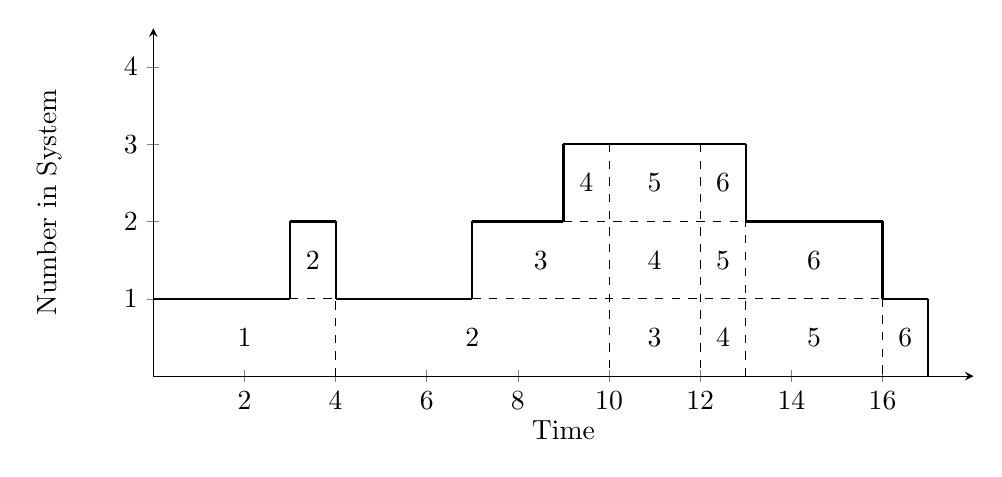
\begin{tikzpicture}[scale=1.0]
    \begin{axis}[clip=false,
      width=12cm, height=6cm,
    axis x line=middle,
    axis y line=middle,
    ymin=0, ymax=4.5,
    ytick={0,1,2,3,4},
    yticklabels={0,1,2,3,4},
    xmin=0, xmax=18,
    xtick={2,4,6,8,10,12,14,16},
    xticklabels={2,4,6,8,10,12,14,16},
    x label style={at={(axis description cs:0.5,-0.1)},anchor=north},
    y label style={at={(axis description cs:-0.1,.5)},rotate=90,anchor=south},
    xlabel=Time,
    ylabel=Number in System,
    ]
    \addplot[mark=none, style=thick] coordinates { (0, 1) (3, 1) };
    \addplot[mark=none, style=thick] coordinates { (3, 1) (3, 2) };
    \addplot[mark=none, style=thick] coordinates { (3, 2) (4, 2) };
    \addplot[mark=none, style=thick] coordinates { (4, 1) (4, 2) };
    \addplot[mark=none, style=thick] coordinates { (4, 1) (7, 1) };
    \addplot[mark=none, style=thick] coordinates { (7, 1) (7, 2) };
    \addplot[mark=none, style=thick] coordinates { (7, 2) (9, 2) };
    \addplot[mark=none, style=thick] coordinates { (9, 2) (9, 3) };
    \addplot[mark=none, style=thick] coordinates { (9, 3) (13,3) };
    \addplot[mark=none, style=thick] coordinates { (13, 3) (13,2) };
    \addplot[mark=none, style=thick] coordinates { (13,2) (16,2) };
    \addplot[mark=none, style=thick] coordinates { (16,2) (16,1) };
    \addplot[mark=none, style=thick] coordinates { (16,1) (17,1) };
    \addplot[mark=none, style=thick] coordinates { (17,1) (17,0) };

    \addplot[mark=none,dashed] coordinates { (3,1) (4,1) };
    \addplot[mark=none,dashed] coordinates { (7,1) (16,1) };
    \addplot[mark=none,dashed] coordinates { (9,2) (13,2) };
    \addplot[mark=none,dashed] coordinates { (10,3) (10,0) };
    \addplot[mark=none,dashed] coordinates { (12,3) (12,0) };
    \addplot[mark=none,dashed] coordinates { (16,1) (16,0) };
    \addplot[mark=none,dashed] coordinates { (4,0) (4,1) };
    \addplot[mark=none,dashed] coordinates { (13,0) (13,2) };

    \node at (2,.5) {1};
    \node at (3.5,1.5) {2};
    \node at (8.5,1.5) {3};
    \node at (9.5,2.5) {4};
    \node at (7,.5) {2};
    \node at (11,.5) {3};
    \node at (11,1.5) {4};
    \node at (11,2.5) {5};
    \node at (12.5,.5) {4};
    \node at (12.5,1.5) {5};
    \node at (12.5,2.5) {6};
    \node at (16.5,.5) {6};
    \node at (14.5,.5) {5};
    \node at (14.5,1.5) {6};

  \end{axis}
\end{tikzpicture}
\end{center}

First note that the problem description does \emph{not} tell us that
the times between arrivals and/or the service times are exponentially
distributed. So it is not an $M/M/1$ system.
The total delay of all six customers is $0+1+3+3+3+4=14$. The average
waiting time in the queue is the total delay divided by the number
of customers.
\[ W_q = \frac{14}{6} = 2.3333~\text{min} \]
To compute the average number in the queue, weight the time in queue
by the number of customers. In other words, compute the area under the
curve but above one, and then divide by the total time.
\[ L_q = \frac{14}{17} \]

\end{solution}

% this problem needs to be re-written.
\item \emph{Justification for a capital expense.}
  Cars arrive at the Lincoln Tunnel toll gate according to a Poisson
  process with an average rate of 90 cars per hour. The time for passing
  the gate is exponential with mean 38 seconds.  Drivers complain of
  the long waiting time, and authorities are willing to reduce the
  average passing time to 30 seconds by installing automatic toll
  collecting devices, provided two conditions are satisfied: 1) the
  average number of waiting cars in the present system exceeds 5 and
  2) the percentage of the gate idle time with the new device
  installed does not exceed 10\%. Can the new device be justified?

\begin{solution}
\bs
Cars arrive at the rate
\[ \lambda = 90~\text{cars per hour} \times 1/3600 =
  1~\text{car}/40~\text{seconds} \]
We know that $\mu=1/38$
for the current system and $\mu_{\text{new}}=1/30$ for the new
system.
Condition 1 states that the average number of waiting
cars in the current system must exceed 5.
\[ L_s = \frac{\lambda}{\mu-\lambda} = \frac{1/40}{1/38-1/40} = 19 \]
You may have also computed
\[ L_q = \frac{\lambda^2}{\mu(\mu-\lambda)} =
  \frac{(1/40)^2}{(1/38)(1/38 - 1/40)} = 18.05 \]
Either way, the first condition is satisfied. The second condition
states that the percentage of idle time in the new system cannot
exceed 10\%.
\[ p_0 = 1 - \frac{\lambda}{\mu_{\text{new}}} = 1 - \frac{1/40}{1/30} = .25 \]
The second condition is not satisfied. There is no justification
for the new toll gate device.
\end{solution}

% this problem needs to be re-written
\item \emph{Comparing system configurations.}
  Pete's Market is a small local grocery store with one checkout counter.
  Shoppers arrive at the checkout lane according to a Poisson process,
  with an arrival rate of 15 customers per hour. The checkout service times
  are distributed Exponential with a service rate of 20 customers per hour.
  The manager is considering two options for improving service.
  \begin{compactenum}
    \item Hire a second person to bag groceries while the cashier is scanning
      and collecting money from the customer. With this improved single-server
      operation, the service rate would be increased to 30 customers per hour.
    \item Hire a second person to operate a second checkout counter. The
      two-server operation would have a service rate of 20 customers per
      hour for each server.
  \end{compactenum}
  Determine the improvements that would result, consider the
  relative cost of each option, and make a recommendation to the manager.

\begin{solution}
\bs Let's look at the average number in the queue $L_Q$ and the
average time in queue $W_Q$ as metrics to judge improvement in
system performance. Because the interarrival times and the service
times are exponentially distributed, we can use the results from
section 11.2. Before any improvements are made,
\[ L_q = \frac{\lambda^2}{\mu(\mu-\lambda)} = \frac{15^2}{20(20-15)} = 2.25~\text{cust} \]
and
\[W_q = \frac{L_q}{\lambda} = \frac{2.25}{15} = .15~\text{hour} = 9~\text{min} \]
If they add a second person to the existing single checkout
\[ L_q = \frac{\lambda^2}{\mu(\mu-\lambda)} = \frac{15^2}{30(30-15)} = 0.5~\text{cust} \]
and
\[W_q = \frac{L_q}{\lambda} = \frac{0.5}{15} = 0.0333~\text{hour} = 2~\text{min} \]
and if they add a completely separate second checkout then we
need to use the formulas from section 11.3 for a two-server operation. First,
\[ P_0 = \frac{1}{\sum_{n=0}^{k-1}\frac{\left(\lambda/\mu\right)^n}{n!} + \frac{\left(\lambda/\mu\right)^k}{k!}\left(\frac{k\mu}{k\mu-\lambda}\right)} \]
where $k=2$ servers. Then
\[ L_q = \frac{\left(\lambda/\mu\right)^k\lambda\mu}{(k-1)!(k\mu-\lambda)^2}P_0 \]
and
\[W_q = \frac{L_q}{\lambda}  \]
Plugging values, I got $P_0=0.4545$, $L_q=0.123$, and $W_q=0.0082$ hours or 0.5 minutes.
Considering the relative improvement and the cost
of adding a second checkout, I would recommend option a). That is, to
add a second person to the existing checkout. The average number in
queue and the average time in queue appear to be acceptable for a
grocery store.
\end{solution}


\end{enumerate}
